
\begin{frame}
\frametitle{Generative models for classification}
\begin{columns}[c]
\column{0.5\textwidth}
\begin{align*}
P(y\!=\!k|{\bf x}) = \frac{P(y\!=\!k) p({\bf x}|y\!=\!k)}{\sum_j P(y\!=\!j) p({\bf x}|y\!=\!j)}
\end{align*}
\column{0.5\textwidth}
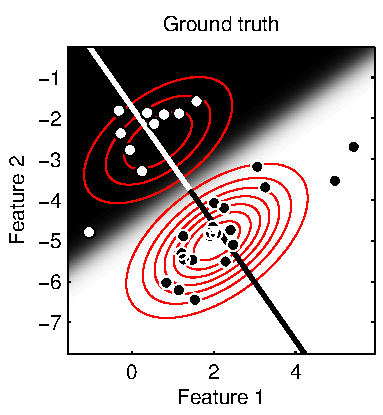
\includegraphics[width=\textwidth]{simple_ground_truth}
\end{columns}
\end{frame}

\begin{frame}
\frametitle{Linear discriminant analysis}
\begin{columns}[c]
\column{0.5\textwidth}
\begin{align*}
P(y\!=\!k|{\bf x}) = \frac{P(y\!=\!k) p({\bf x}|y\!=\!k)}{\sum_j P(y\!=\!j) p({\bf x}|y\!=\!j)}
\end{align*}
Assumes:
\begin{align*}
P({\bf x}|y\!=\!k) = \mathcal{N}({\bf x} | {\boldsymbol\mu}_k, \boldsymbol\Sigma)
\end{align*}
\column{0.5\textwidth}
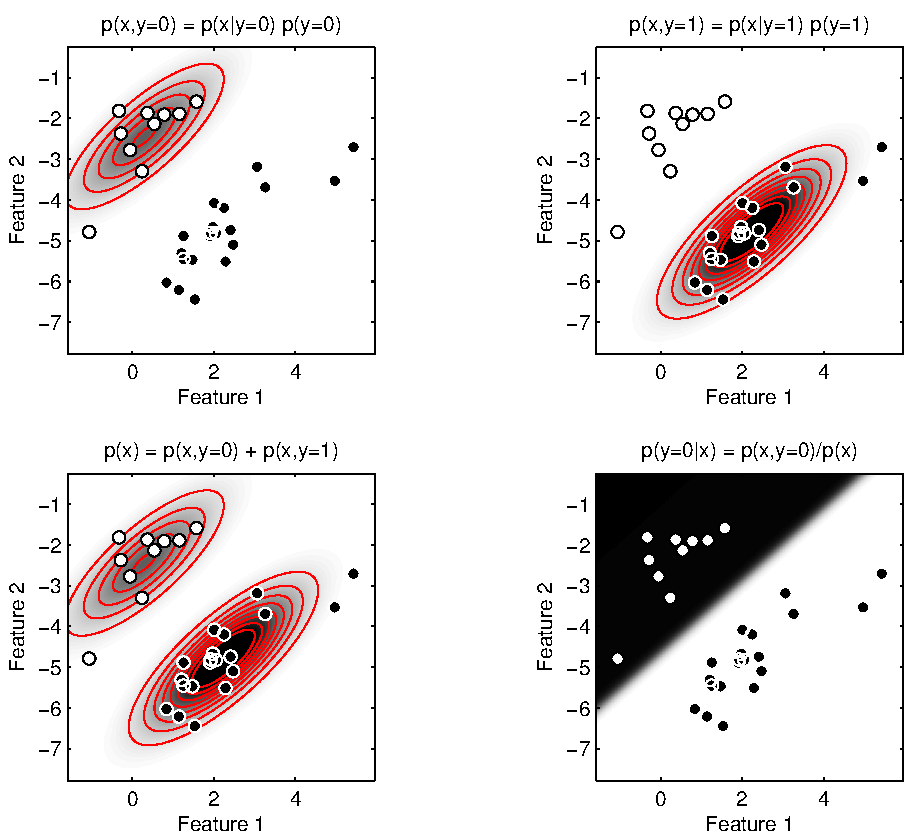
\includegraphics[width=\textwidth]{simple_fld}
\end{columns}
Model has $2p + p(p-1)$ parameters to estimate (two means and a single covariance).\par
Number of observations is $pn$ (size of inputs).
\end{frame}

\begin{frame}
\frametitle{Quadratic discriminant analysis}
\begin{columns}[c]
\column{0.5\textwidth}
\begin{align*}
P(y\!=\!k|{\bf x}) = \frac{P(y\!=\!k) p({\bf x}|y\!=\!k)}{\sum_j P(y\!=\!j) p({\bf x}|y\!=\!j)}
\end{align*}
Assumes different covariances:
\begin{align*}
P({\bf x}|y\!=\!k) = \mathcal{N}({\bf x} | {\boldsymbol\mu}_k, {\boldsymbol\Sigma}_k)
\end{align*}
\column{0.5\textwidth}
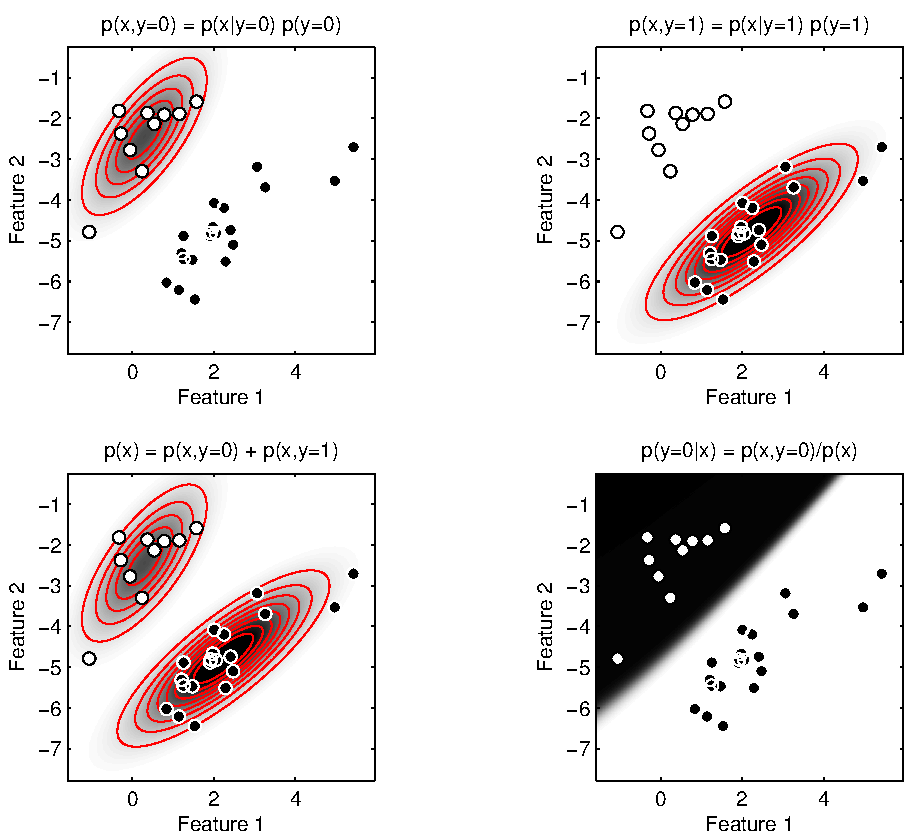
\includegraphics[width=\textwidth]{simple_qda}
\end{columns}
Model has $2p + 2p(p-1)$ parameters to estimate (two means and two covariances).\par
Number of observations is $pn$.
\end{frame}

\begin{frame}
\frametitle{Naive Bayes}
\begin{columns}[c]
\column{0.5\textwidth}
\begin{align*}
P(y\!=\!k|{\bf x}) = \frac{P(y\!=\!k) p({\bf x}|y\!=\!k)}{\sum_j P(y\!=\!j) p({\bf x}|y\!=\!j)}\cr
\end{align*}
Assumes that features are independent:
\begin{align*}
p({\bf x}|y\!=\!k) = \prod_i p(x_i|y\!=\!k)
\end{align*}
\column{0.5\textwidth}
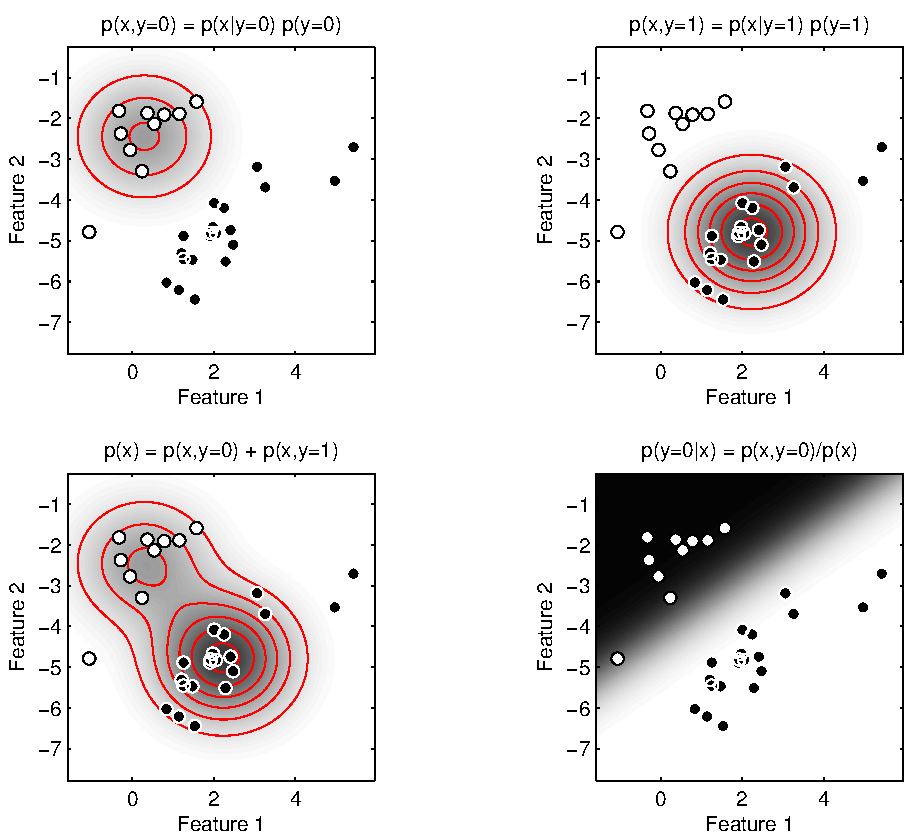
\includegraphics[width=\textwidth]{simple_naive_bayes}
\end{columns}
Model has variable number of parameters to estimate, but the above example has $3p$.\par
Number of observations is $pn$.
\end{frame}

